\chapter{Phase Transitions and Critical Phenomena}
\label{ch:crit}

When trying to analyze a physical system, a big part of a physicist effort is
dedicated to identifying the parts that compose the system and how they
interact with each other. It is usually a daunting task to find an interaction
model that captures all the expected properties of a system. That's because the
macroscopic (i.e.\ collective) behavior does not follow trivially from the
microscopic forces in place. In no area of physics this is more clear than in
that of phase transitions and critical phenomena. Not surprisingly the
relationship between criticality and complexity has been applied to areas well
beyond the domain of atoms and molecules, like cognitive
sciences~\cite{Kello2010}, social scieces~\cite{Kron2009} and
ecology~\cite{Sole1999}, to name just a few.

But let's take a step back and look at the components themselves. We can get
away with making very little assumptions about their actual identities. They
can be elementary particles when studying high energy physics, atoms and
molecules when determining the electronic properties of a material, living
cells when observing the growing pattern of a colony of bacteria, or even
people when trying to design buildings with safe exit routes. What is more
important to us is the fact that these building blocks can organize themselves
in several different ways. Each pattern of organization is called a
\textit{phase}, and in which phase the systems finds itself depends on the
value of some external parameter, like energy density, temperature, nutrient
concentration or whether or not there's a fire in the building. Not only that
but different phases of a same system display wildly different macroscopic
behavior, despite no change taking place in their composition.

The most familiar example is water. At sea level, water is in its solid phase
for temperatures lower than $0^\circ$C. That happens because the water
molecules are locked in place by the cohesive forces that its neighbors exert
on each other. When the temperature is higher than $0^\circ$C but lower than
$100^\circ$C, the molecules acquire enough kinetic energy to be able to move
through one another. They still interact strongly enough to be bound together
but it is not sufficient to keep them fixed. This is the liquid phase. When the
temperature is above $100^\circ$C, water is now in the gaseous state, where
thermal movement dominates the dynamics of the system. The molecules
now move mostly unimpeded, interacting only when colliding directly. See
Fig.~\ref{fig:phases} for an illustration of how a molecule moves in the three
phases.

Not all phases concern the states of matter, however. Some are related to
magnetic or electric properties. This is the case of ferromagnetic materials,
materials that exhibit a persistent magnetization after being subject to a
strong magnetic field, like your everyday fridge magnet. In contrast,
paramagnetic materials show no permanent magnetization. Ferromagnetism is a
result of the alignment of the magnetic spins of the atoms that compose the
material. If you turn off the external field and raise the temperature,
eventually the thermal fluctuations will misalign the spins, zeroing out the
magnetization and turning a ferromagnetic material into a paramagnetic one.

To better visualize the different phases of systems, it is common to make use
of a \textit{phase diagram}. Simply put, a phase diagram is a graph where each
axis represent one control parameter, and every point in this graph is labeled
according to the phase the system finds itself for that value of the
parameters. Figure~\ref{fig:water}a shows the very famous phase diagram of
water as a function of temperature and pressure. The three main phases (solid,
liquid and gas) are clearly marked, and the black lines are the boundary
between the phases. Crossing any of these lines is followed by a sharp change
on the properties of the system, as described previously. This is know as a
\textit{phase transition}.

\begin{figure}[h]
\begin{center}
    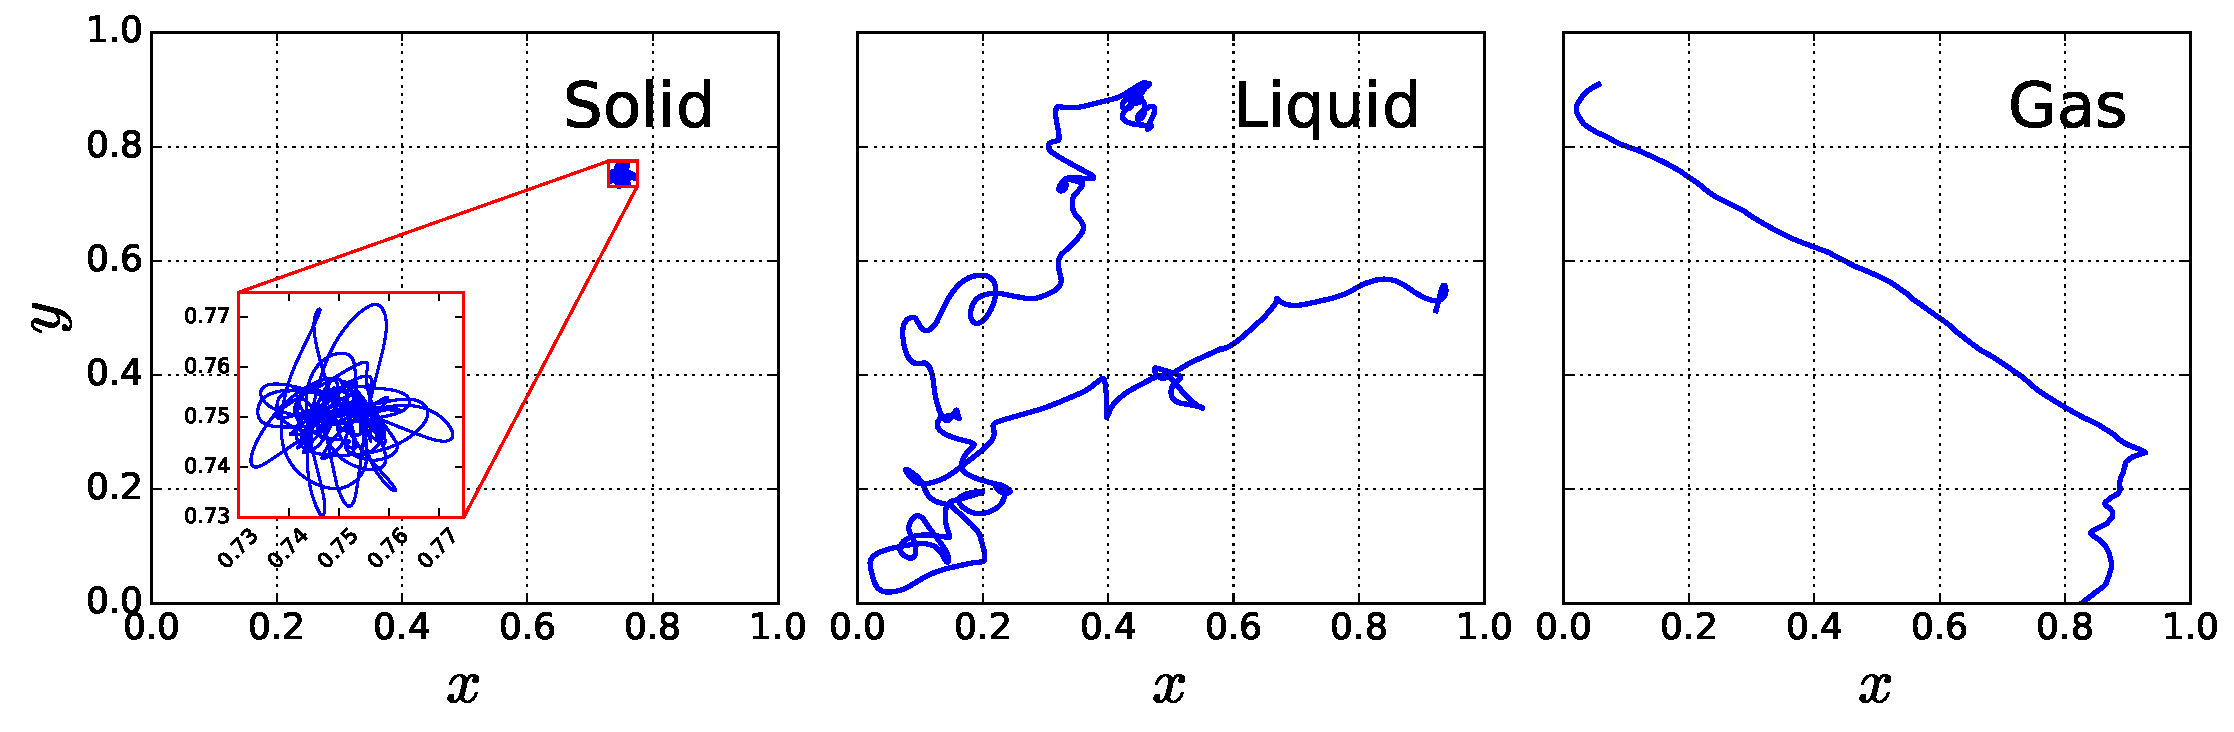
\includegraphics[scale=0.4]{chapters/ch2-crit/figs/phases}
\end{center}
\caption{How a system of particles behave in the three phases of matter. Here a
    simulation of 100 particles was done, but the trajectory of only one is
    shown. In the solid state the particles are confined to small region by
    the interactions of its neighbors. In the liquid state the particle is
    unconfined, but still interacts strongly with the other particles. In the
    gas state the kinetic energy of the particles is large enough that they
    barely interact with one another, making a ballistic trajectory until
    they make a head-on collision with another particle.}
\label{fig:phases}
\end{figure}


\begin{figure}[h]
\begin{center}
    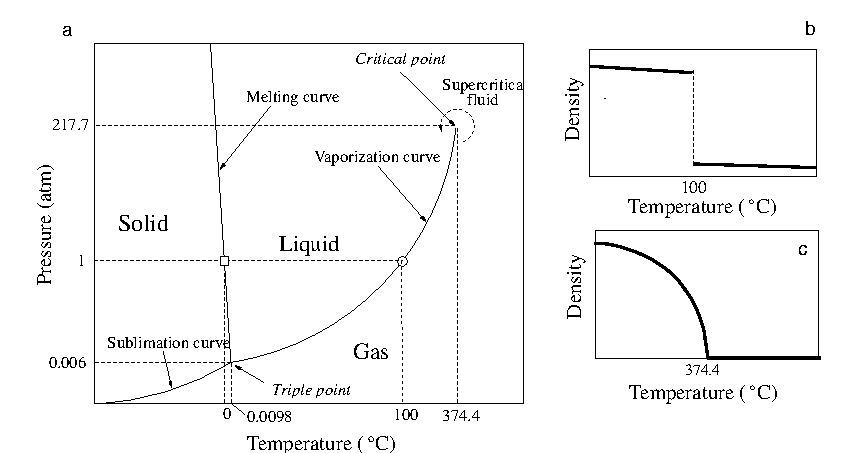
\includegraphics[scale=1.0]{chapters/ch2-crit/figs/water}
\end{center}
\caption{Phase diagram of water (a). Here, the three usual phases are
    distinguished, each separated from the other by a critical line. The phase
    transition that happens when the system traverse a line is characterized by
    a discontinuous jump in the density, as shown in (b) for the liquid-gas
    transition at $P=1$ atm. For $P=217.7$ atm however the same transition is
    continuous, as shown in (c). In the vicinity of this phase transition, at
    $T\approx374.4^\circ$C, the two phases become indistinguishable, and
    display a number of peculiarities. Systems in such state are called
    critical systems. Reproduced from~\cite{Sole2011}.}
\label{fig:water}
\end{figure}


\section{Classification of Phase Transitions}
\label{sec:classification}

Phase transitions are usually classified into two categories: first and second
order. There's no consensus on the precise definition of each, but this does
not matter a lot, since they behave quite differently. An old, but still often
used definition was proposed by Ehrenfest~\cite{Jaeger1998}. But, before we get
into that, we have to find a quantitative way of describing the phase of a
system. This is done by defining an \textit{order parameter}, a quantity that
take very distinct values in different phases (usually normalized to be zero in
the high temperature phase). In the case of water, the order parameter is the
density or, equivalently, the volume. For ferromagnetic transitions we use the
spontaneous magnetization.

Following the example of water, where the temperature and pressure are the
control variables, the thermodynamic properties are determined by it's Gibbs
free energy
\begin{equation}
    G=E-TS+pV.
\end{equation}
from which we can obtain the volume by taking its derivative
\begin{equation}
    V={\left(\frac{\partial G}{\partial p}\right)}_T.
\end{equation}
If we now make an experimental apparatus to try and observe the behavior of the
density of an amount of water during a phase transition, say the liquid-gas
transition, what we see is show in Figure~\ref{fig:water}b. The density (and
therefore the volume) makes a discontinuous jump. Less evident, but no less
true, is that the entropy, another derivative of $G$,
\begin{equation}
    S=-{\left(\frac{\partial G}{\partial T}\right)}_p,
\end{equation}
is also discontinuous at the boundary of a phase transition. Because the first
derivatives of the free energy display a singularity, we say these phase
transition are of \textit{first order}. This sudden changes happens because the
equilibrium state of the system (the minimum of the free energy) shifts from
one part of the phase space to another~\cite{Callen1985} as illustrated in
Figure~\ref{fig:gibbs1}. When the system is exactly at the boundary of the
phase transition, both phases have the same free energy, allowing them both to
coexist in different regions of the system. Because of this, the transition
lines are also called coexistence lines.

\begin{figure}[h]
\begin{center}
    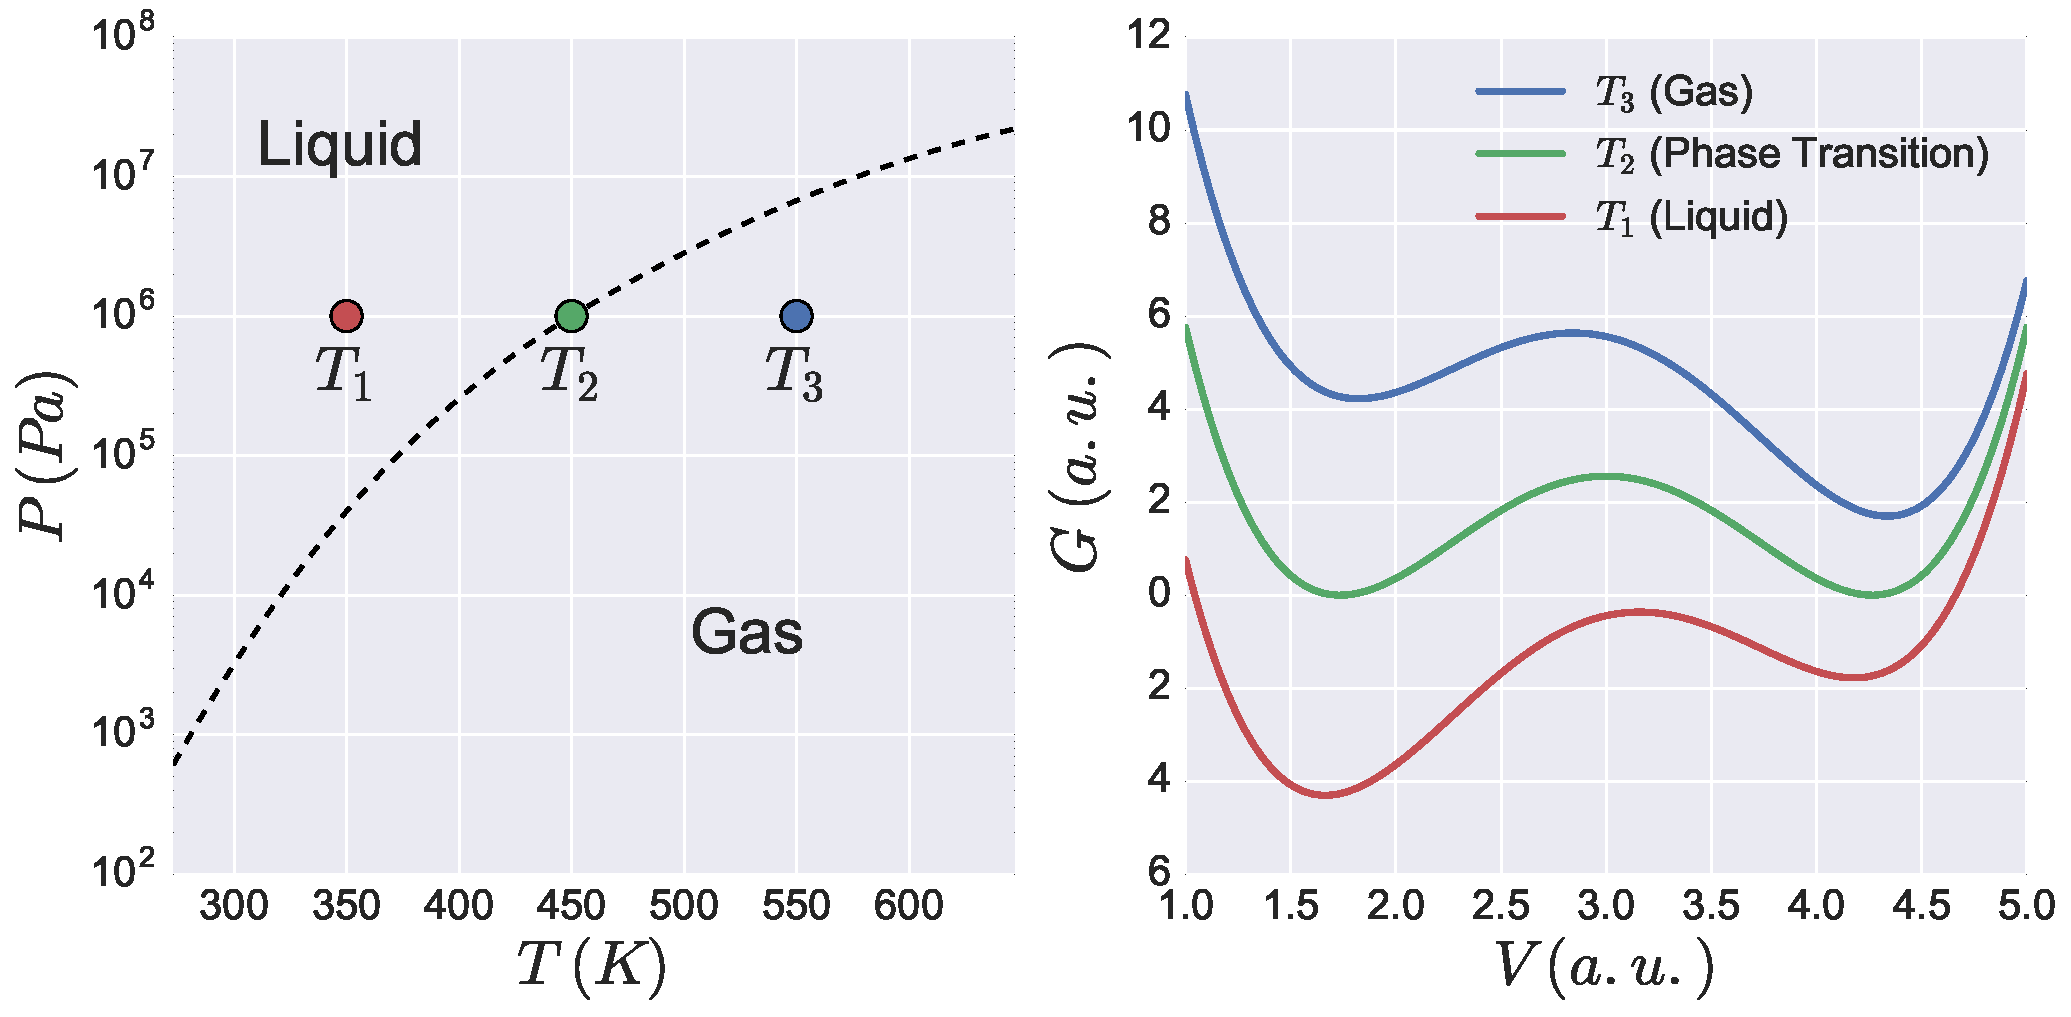
\includegraphics[scale=0.4]{chapters/ch2-crit/figs/gibbs1}
\end{center}
\caption{Why first order transitions happen. The left graph shows three points
    on the phase space of water. The red one is in the liquid phase, the blue
    is in the gaseous state and the green right on the boundary. The right
    graph shows a heuristic construction of the Gibbs free energy in each of
    the three points (matched by color). The equilibrium state is the one of
    minimal free energy. Although $G$ changes continuously with the
    temperature, the global minimum shifts abruptly once the phase boundary is
    crossed, thus occurring a first order phase transition. When the system is
    exactly on the boundary, the minima are equivalent, and the two phases
    coexist.}
\label{fig:gibbs1}
\end{figure}


First order transitions are characterized by the presence of latent heat, an
amount of energy that the system releases or absorbs during a phase transition,
which is a constant of the substance, and is independent on the temperature,
pressure or other control parameter~\cite{Callen1985}. This means that when
boiling a volume of water, the temperature of the liquid phase does not rise
because the extra heat being added is being absorbed in form of latent heat.

Looking again at Figure~\ref{fig:water}a one might ask why the liquid-gas
transition line does not extend for all values of temperature. This is where
things start to get interesting. We've established that the free energy have
two equivalent minima when the system is over the coexistence line. Now, if we
walk along this line following the behavior of the free energy, what we observe
is something similar to what is shown in Figure~\ref{fig:gibbs2}. At a
temperature of approximately $374^\circ$C and pressure of $217.7$atm, the two
minima join into one. At this point it is not that the two phases coexist, they
are indistinguishable.

If we look at the order parameter of the systems when it goes through the
critical point, we see that the transition is no longer discontinuous, as it's
shown in Figure~\ref{fig:water}c. If we set the pressure to the same as the
critical point and heat an amount of liquid water, the volume will rise
continuously until it reaches the gaseous state. We can observe the behavior of
other thermodynamic quantities near the critical point, like the specific heat
\begin{equation}
    c_p=T{\left(\frac{\partial S}{\partial T}\right)}_{p}=
    T{\left(\frac{\partial^{2}G}{\partial T^{2}}\right)}_{p},
\end{equation}
or the isothermal compressibility
\begin{equation}
    \kappa_T=-\frac{1}{V}{\left(\frac{\partial V}{\partial p}\right)}_{T}=
    -\frac{1}{V}{\left(\frac{\partial^{2}G}{\partial p^{2}}\right)}_{T},
\end{equation}
What we see is a very clear divergence near the critical point. Because these
diverging quantities are second derivatives of the free energy, we say this is
a \textit{second order} phase transition, and systems close to the critical
point are called \textit{critical systems}.

Second order transitions have a whole range of peculiar behavior associated
with it. The most notorious is the presence of large fluctuations. In
Chapter~\ref{ch:intr} we mentioned the work of Thomas
Andrews~\cite{Andrews1869}, who noticed that some substances become opaque at
the critical point. This happens because of the huge fluctuations in the
density of the systems, which are present in all size scales, scattering most
visible light.

The ferromagnetic transition described in the previous section is probably the
most studied kind of second order phase transition. In it the free energy is
given by
\begin{equation}
    F = -SdT-Mdh
\end{equation}
where $M$ is the spontaneous magnetization and $h$ is an external magnetic
field. It is characterized by a diverging magnetic susceptibility
\begin{equation}
    \chi_{M}=
    {\left(\frac{\partial M}{\partial h}\right)}_{T}=
    -{\left(\frac{\partial^{2}F}{\partial h^{2}}\right)}_{T}.
\end{equation}

\begin{figure}[h]
\begin{center}
    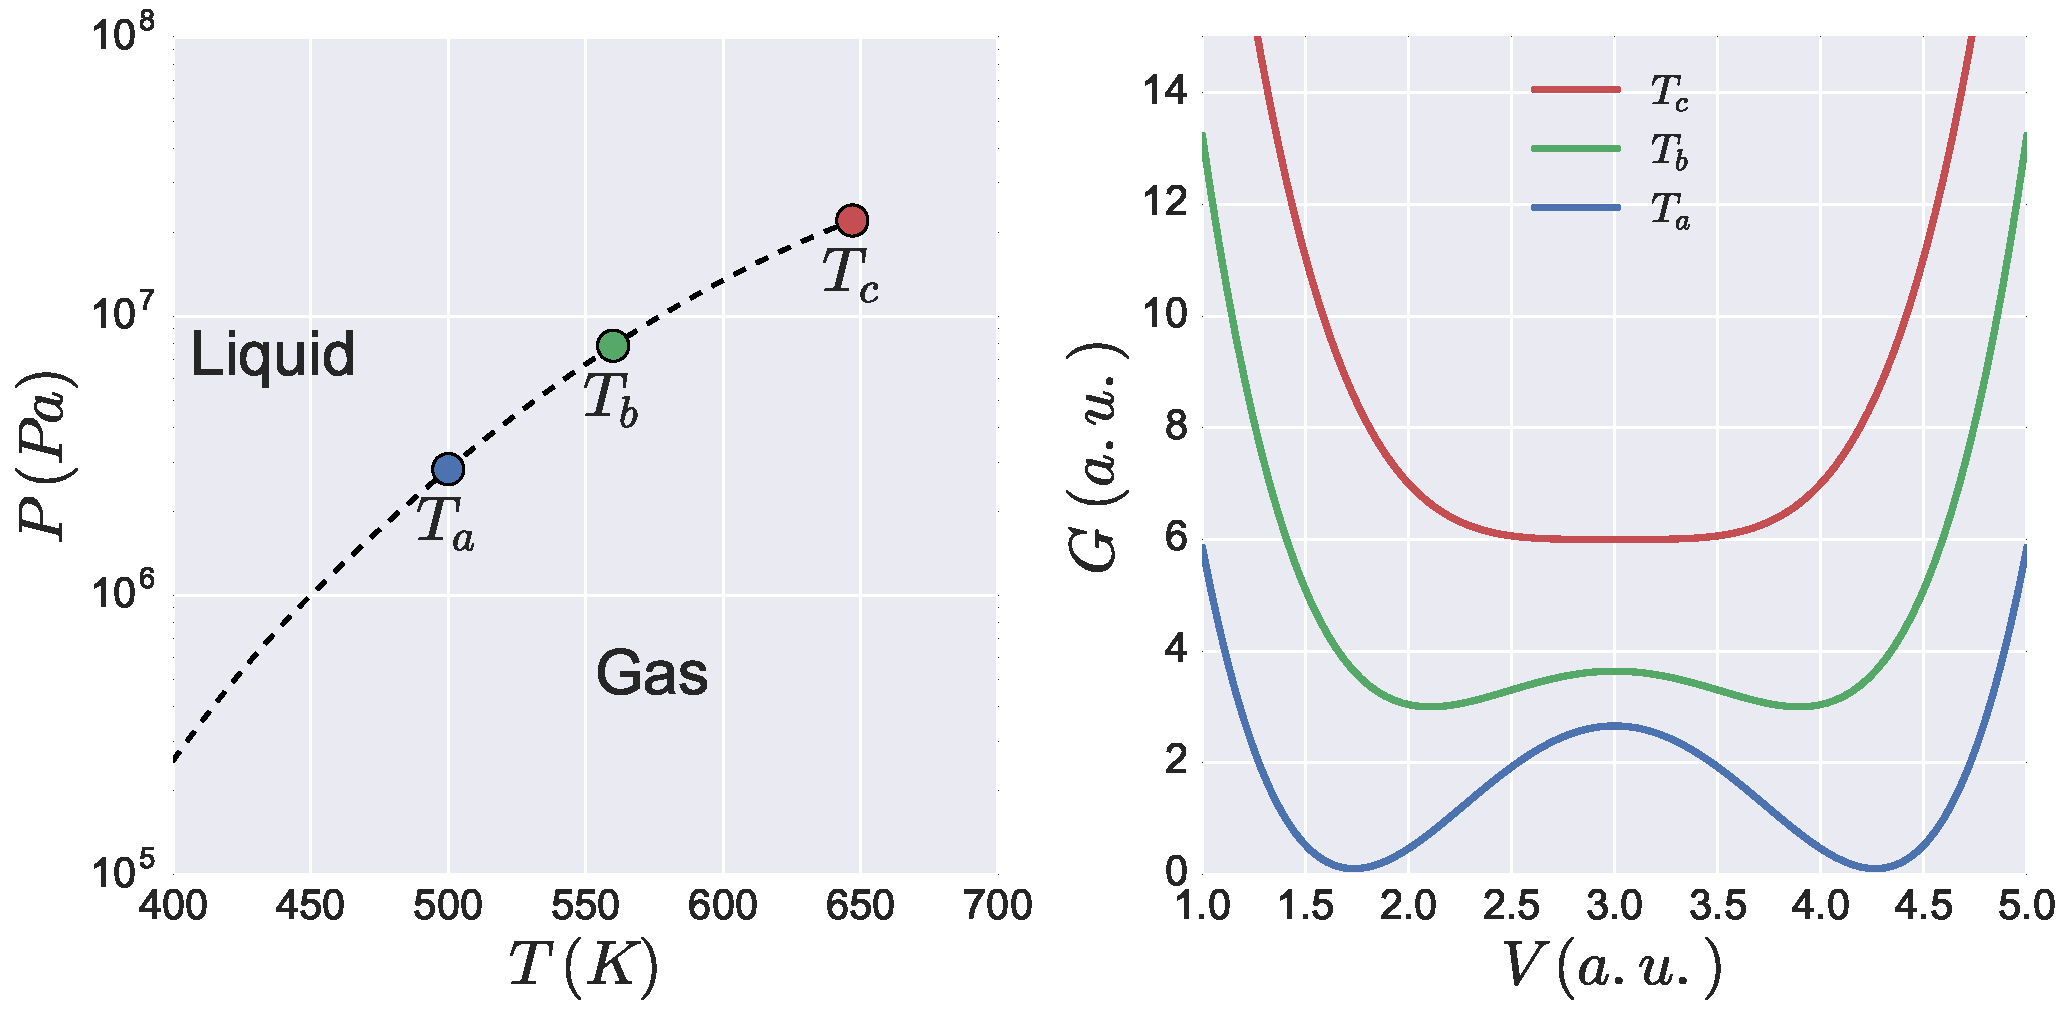
\includegraphics[scale=0.4]{chapters/ch2-crit/figs/gibbs2}
\end{center}
\caption{If we follow the (heuristic) Gibbs free energy along the liquid-gas
    line, we observe that at some critical point $T_c$ the two minima (related
    to the liquid and gas phases) coalesce into one. At this point the two
    phases are indistinguishable, which characterizes a second order phase
    transition. Systems close to the critical point are called critical
    systems.}
\label{fig:gibbs2}
\end{figure}


\begin{figure}[h]
\begin{center}
    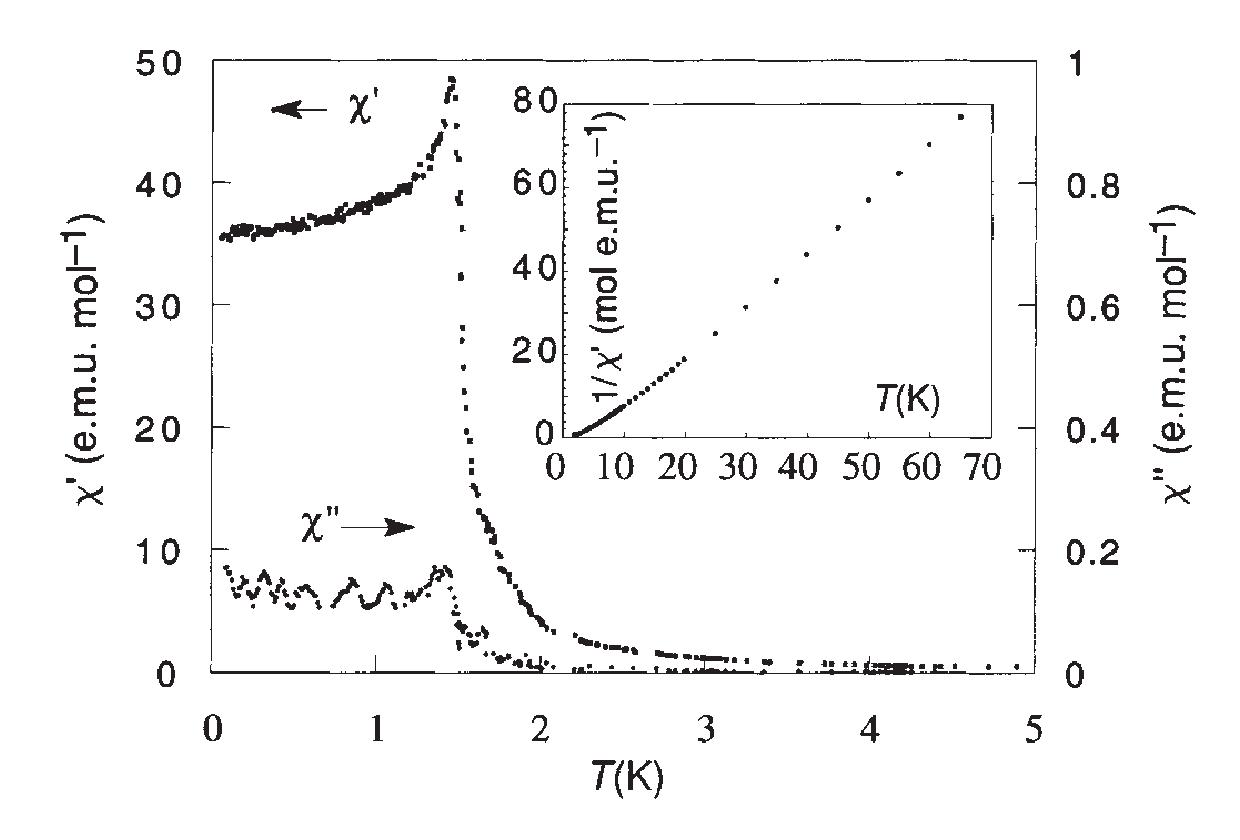
\includegraphics[scale=0.6]{chapters/ch2-crit/figs/suscep}
\end{center}
\caption{Example of a ferromagnetic transition in dupeyredioxyl. The graph
    shows a distinctive divergence in the magnetic susceptibility in the
    vicinity of the critical point $T_c\approx1.48$K. Reproduced
    from~\cite{Chiarelli1993}.}
\label{fig:suscep}
\end{figure}

Not all phase transitions fall neatly into these two categories, however. The
Kosterlitz-Thouless transition of the XY-Model (related to some superconducting
transitions~\cite{Resnick1981}) could be considered of infinite order, because
the free energy is infinitely differentiable~\cite{Kosterlitz1973}, although it
shares a lot of similarities with second order transitions.


\section{Critical Exponents and Universality}
\label{sec:universality}

The discussion of phase transitions presented in the last section, rooted on
the postulates of thermodynamics and in the analyticity of the free energy, is
due to Landau~\cite{Landau1969}. While this theory menages to capture a few
properties 

We noted that several thermodynamical quantities diverge on the critical point.
Not only that, that

There are four basic thermodynamical critical exponents, defined as follows.

The heat capacity exponent $\alpha$
\begin{equation}
    C \sim \left|T-T_c\right|^{-\alpha}.
\end{equation}
The generalized susceptibility exponent $\gamma$
\begin{equation}
    \chi \sim \left|T-T_c\right|^{-\gamma}.
\end{equation}
The order parameter exponent $\beta$, when taken along the coexistence curve 
\begin{equation}
    \Phi \sim {\left|T-T_c\right|}^{\beta}.
\end{equation}
The order parameter exponent $\delta$, when taken at constant temperature
$T=T_c$
\begin{equation}
    \Phi \sim \left|J-J_c\right|^{1/\delta}.
\end{equation}
These exponents may have different values if you take the limit from above or
bellow the critical point, but it should be enough for us to assume they are
the same.

There are many other critical exponents outside the realm of thermodynamics and
well into the statistical mechanics domain.


\section{Models of Critical Systems}
\label{sec:models}

Lorem ipsum dolor sit amet, consectetur adipisicing elit, sed do eiusmod tempor
incididunt ut labore et dolore magna aliqua. Ut enim ad minim veniam, quis
nostrud exercitation ullamco laboris nisi ut aliquip ex ea commodo consequat.
Duis aute irure dolor in reprehenderit in voluptate velit esse cillum dolore eu
fugiat nulla pariatur. Excepteur sint occaecat cupidatat non proident, sunt in
culpa qui officia deserunt mollit anim id est laborum.

\subsection{Ising Model}
\label{sec:ising}

Although not directly relevant for the present work, we shall describe briefly
the Ising model if only because of its importance in the field of critical
phenomena.


\subsection{Percolation}
\label{sec:perc}

While the Ising model certainly wins in terms of popularity, very few models
match the simplicity of percolation. Introduced in 1957 by Broadbent and
Hammersley, the passing decades saw its rise in prominence due to it's high
applicability ranging from transport in porous media to the propagation of
infectious diseases, with pretty much everything in between~\cite{Araujo2013}.
